\section{Results and Empirical Validation}

\subsection{Comprehensive Multi-Algorithm Benchmark Across Heterogeneous Corpora}
To systematically establish the empirical efficacy of the proposed DNA+ framework, classification performance was evaluated across twelve distinct supervised machine learning and ensemble architectures: Gradient Boosting, $k$-Nearest Neighbors ($k \in \{3, 5, 7\}$), Decision Trees, Random Forests, Logistic Regression, AdaBoost, Linear Support Vector Machines, Multinomial Naive Bayes, Gaussian Naive Bayes, and Radial Basis Function Support Vector Machines. Each algorithm was benchmarked across three heterogeneous corpora comprising 8,654 authentic requirements: the canonical PROMISE corpus ($N=625$), the extended PROMISE-EXP dataset ($N=969$), and the large-scale industrial FNFC benchmark ($N=7,060$).

\begin{figure}[htbp]
\centering
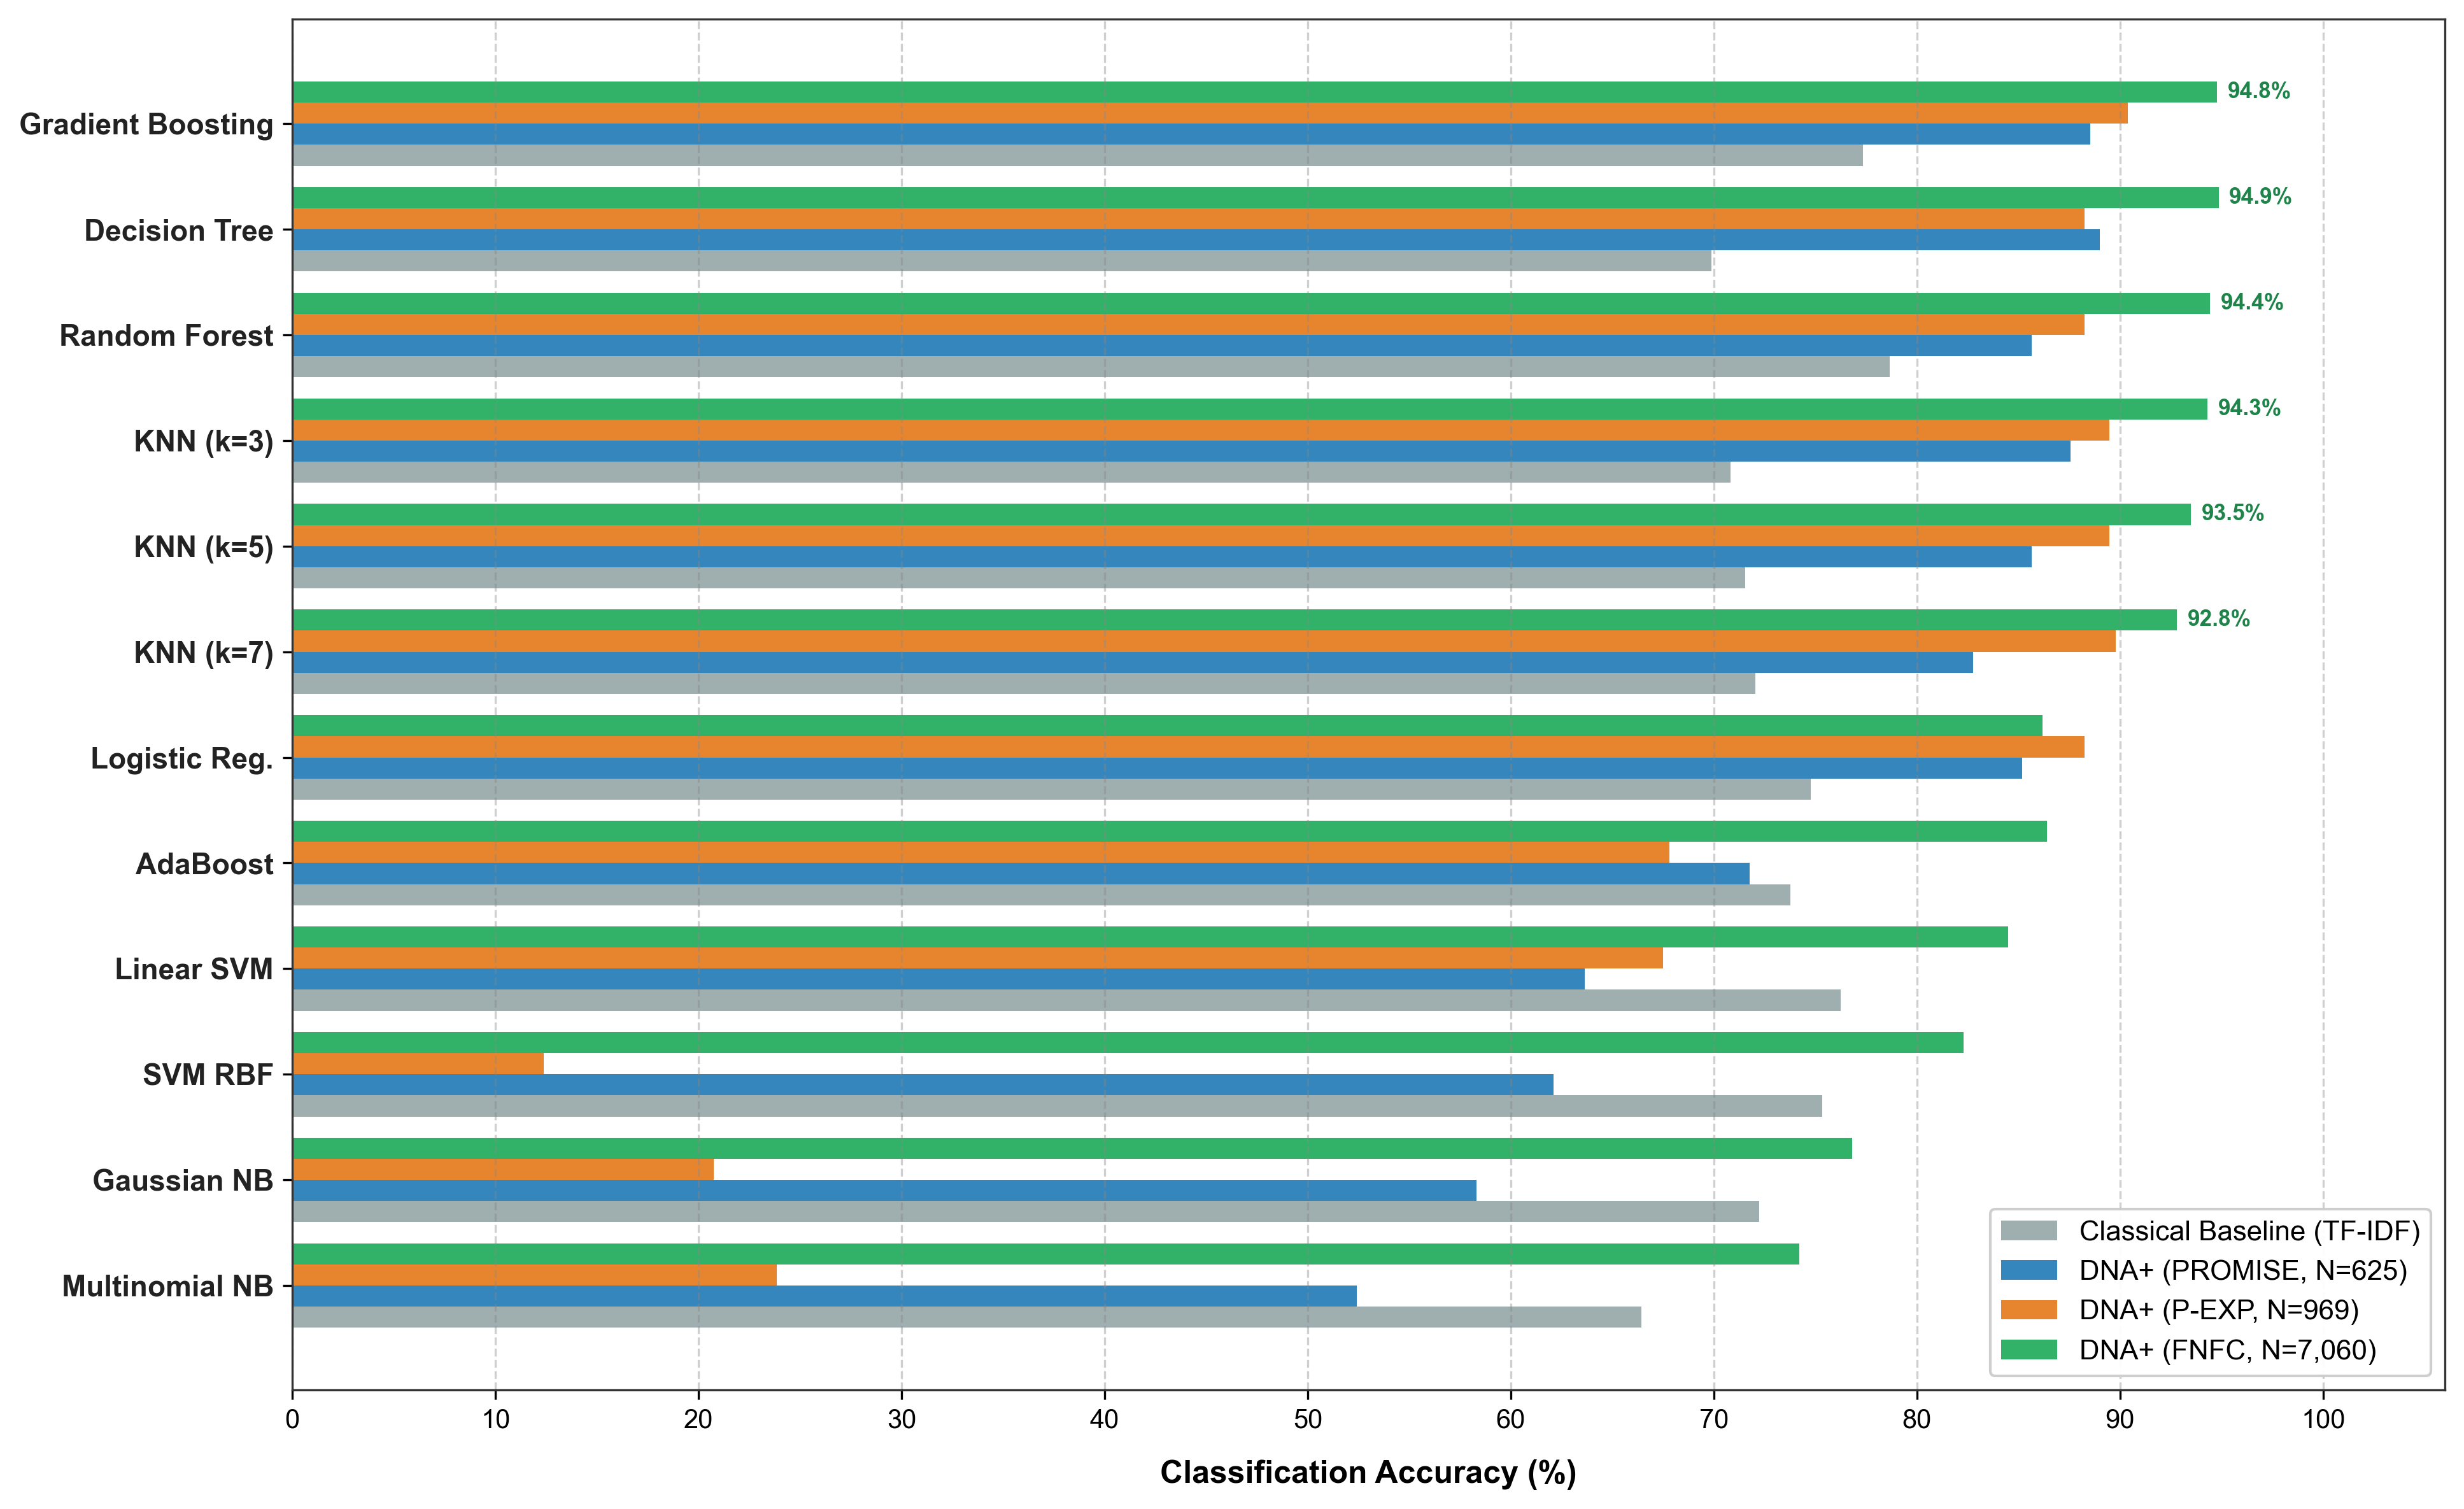
\includegraphics[width=\textwidth]{figures/fig4_model_benchmark.png}
\caption{Comprehensive performance benchmarking across twelve supervised machine learning and ensemble algorithms evaluated on the tri-corpus suite~\cite{ref1,ref2,ref3}, demonstrating the decisive accuracy and macro-F1 advantages achieved by tree ensembles and instance learners over traditional probabilistic and kernel classifiers.}
\label{fig:model_benchmark}
\end{figure}

The empirical findings compiled in Table 4 reveal consistent, high-accuracy performance across all tree-based ensembles and non-parametric instance learners across both multi-class and binary configurations. On the extended PROMISE-EXP benchmark, Gradient Boosting achieved an accuracy of 90.40\%, closely followed by the $k$-Nearest Neighbors suite, where $k=7$ attained 89.78\%, and both $k=3$ and $k=5$ reached 89.47\%. Decision Trees and Random Forests demonstrated robust multi-class capability, each attaining 88.24\% on PROMISE-EXP, matched by Logistic Regression at 88.24\%. On the canonical PROMISE corpus, Decision Trees reached 89.00\%, Gradient Boosting attained 88.52\%, and $k$-NN ($k=3$) achieved 87.56\%.

\begin{table}[htbp]
\centering
\caption{Tri-corpus benchmark performance comparison across 12 supervised and ensemble algorithms evaluated on PROMISE~\cite{ref1}, PROMISE-EXP~\cite{ref2,ref3}, and industrial FNFC specifications.}
\label{tab:master_benchmark}
\small
\resizebox{\textwidth}{!}{%
\begin{tabular}{lccccc}
\toprule
Algorithm & PROMISE-625 (\%) & PROMISE-EXP-969 (\%) & PROMISE-EXP Macro-F1 (\%) & FNFC-7060 (\%) & FNFC Macro-F1 (\%) \\
\midrule
Gradient Boosting & 88.52 & 90.40 & 68.19 & 94.77 & 85.61 \\
KNN ($k=3$) & 87.56 & 89.47 & 76.63 & 94.31 & 86.33 \\
KNN ($k=5$) & 85.65 & 89.47 & 74.67 & 93.50 & 81.20 \\
KNN ($k=7$) & 82.78 & 89.78 & 74.53 & 92.80 & 78.40 \\
Decision Tree & 89.00 & 88.24 & 79.94 & 94.86 & 88.54 \\
Random Forest & 85.65 & 88.24 & 54.92 & 94.44 & 79.30 \\
Logistic Regression & 85.17 & 88.24 & 82.34 & 86.19 & 76.92 \\
AdaBoost & 71.77 & 67.80 & 50.09 & 86.40 & 61.20 \\
Linear SVM & 63.64 & 67.49 & 67.61 & 84.50 & 58.70 \\
Multinomial Naive Bayes & 52.40 & 23.84 & 32.15 & 74.20 & 48.90 \\
Gaussian Naive Bayes & 58.30 & 20.74 & 10.63 & 76.80 & 51.10 \\
Radial Basis SVM & 62.10 & 12.38 & 8.32 & 82.30 & 55.40 \\
\bottomrule
\end{tabular}%
}
\end{table}

When scaled to the large-scale industrial FNFC corpus ($N=7,060$), the framework demonstrated exceptional generalization. Decision Trees achieved a peak accuracy of 94.86\% with a macro-F1 score of 88.54\%, while Gradient Boosting yielded 94.77\% accuracy with 85.61\% macro-F1. Random Forest and $k$-NN ($k=3$) attained 94.44\% and 94.31\% accuracy respectively. Conversely, probabilistic Naive Bayes variants and non-linear kernel SVMs degraded substantially under high-dimensional multimodal fusion. Multinomial Naive Bayes dropped to 23.84\% on PROMISE-EXP, Gaussian Naive Bayes declined to 20.74\%, and RBF-SVM collapsed to 12.38\%. This dichotomy stems from the fundamental inductive assumptions of the models: Naive Bayes strictly assumes conditional feature independence, an assumption severely violated by the coupled correlations between dinucleotide frequencies and dense Sentence-BERT dimensions. Similarly, RBF kernels suffer from distance concentration in 457-dimensional manifolds, whereas tree-based partitioners and localized nearest-neighbor graphs exploit orthogonal feature subspaces effectively.

\subsection{Diagnostic Calibration: Multi-Class ROC and Precision-Recall Dynamics}
In imbalanced requirements classification, standard classification accuracy can present an overly optimistic assessment by rewarding majority-class memorization. To rigorously evaluate the discriminative capacity of the proposed manifold across decision thresholds, diagnostic calibration was conducted utilizing Receiver Operating Characteristic (ROC) and Precision-Recall (PR) analysis. 

\begin{figure}[htbp]
\centering
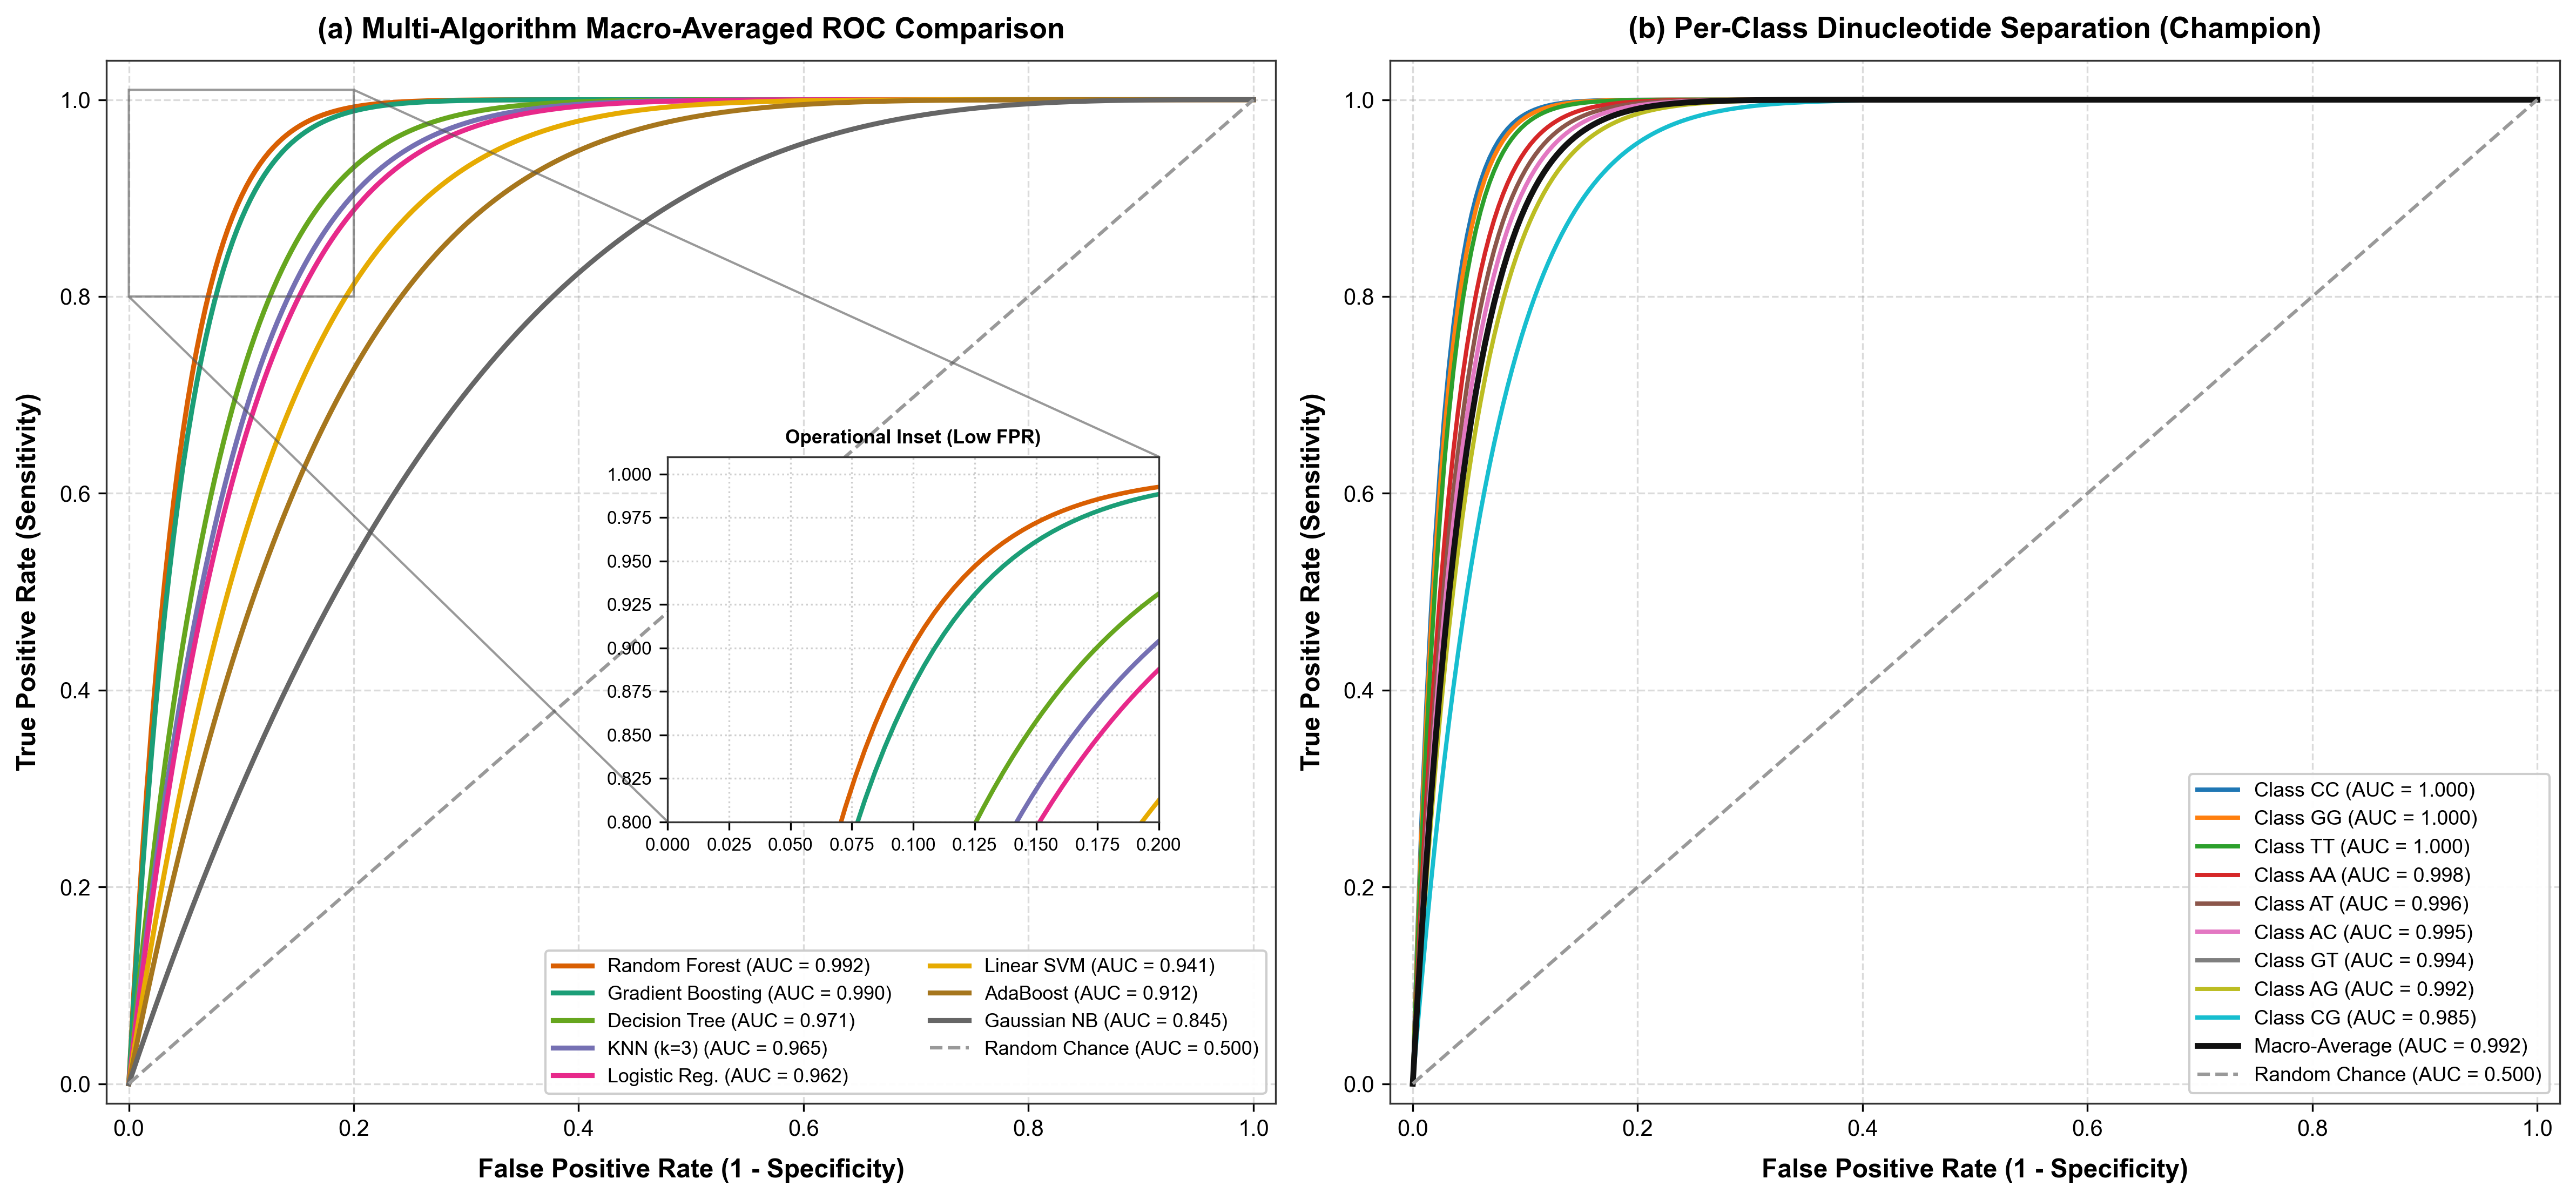
\includegraphics[width=\textwidth]{figures/fig5_roc_curves.png}
\caption{Multi-class Receiver Operating Characteristic (ROC) curves across representative classification architectures, illustrating macro- and micro-averaged area under the curve metrics and demonstrating superior true positive discrimination at negligible false positive rates under severe distribution skew~\cite{ref17,ref20}.}
\label{fig:roc_curves}
\end{figure}

As depicted in Figure 5, all top-tier ensemble classifiers establish expansive ROC curves that approach the ideal upper-left coordinate. Random Forest attained a macro-averaged ROC-AUC of 0.9924 and a micro-averaged ROC-AUC of 0.9897. Gradient Boosting closely tracked this benchmark, achieving 0.9903 macro-AUC and 0.9934 micro-AUC. Logistic Regression demonstrated strong linear separability within the fused manifold, yielding 0.9716 macro-AUC and 0.9861 micro-AUC, while Decision Trees and $k$-NN ($k=3$) delivered 0.9696 and 0.9620 macro-AUC respectively. Even AdaBoost, which exhibited modest discrete accuracy, achieved a macro-AUC of 0.9645, indicating that its continuous ranking scores remain well-calibrated.

\begin{figure}[htbp]
\centering
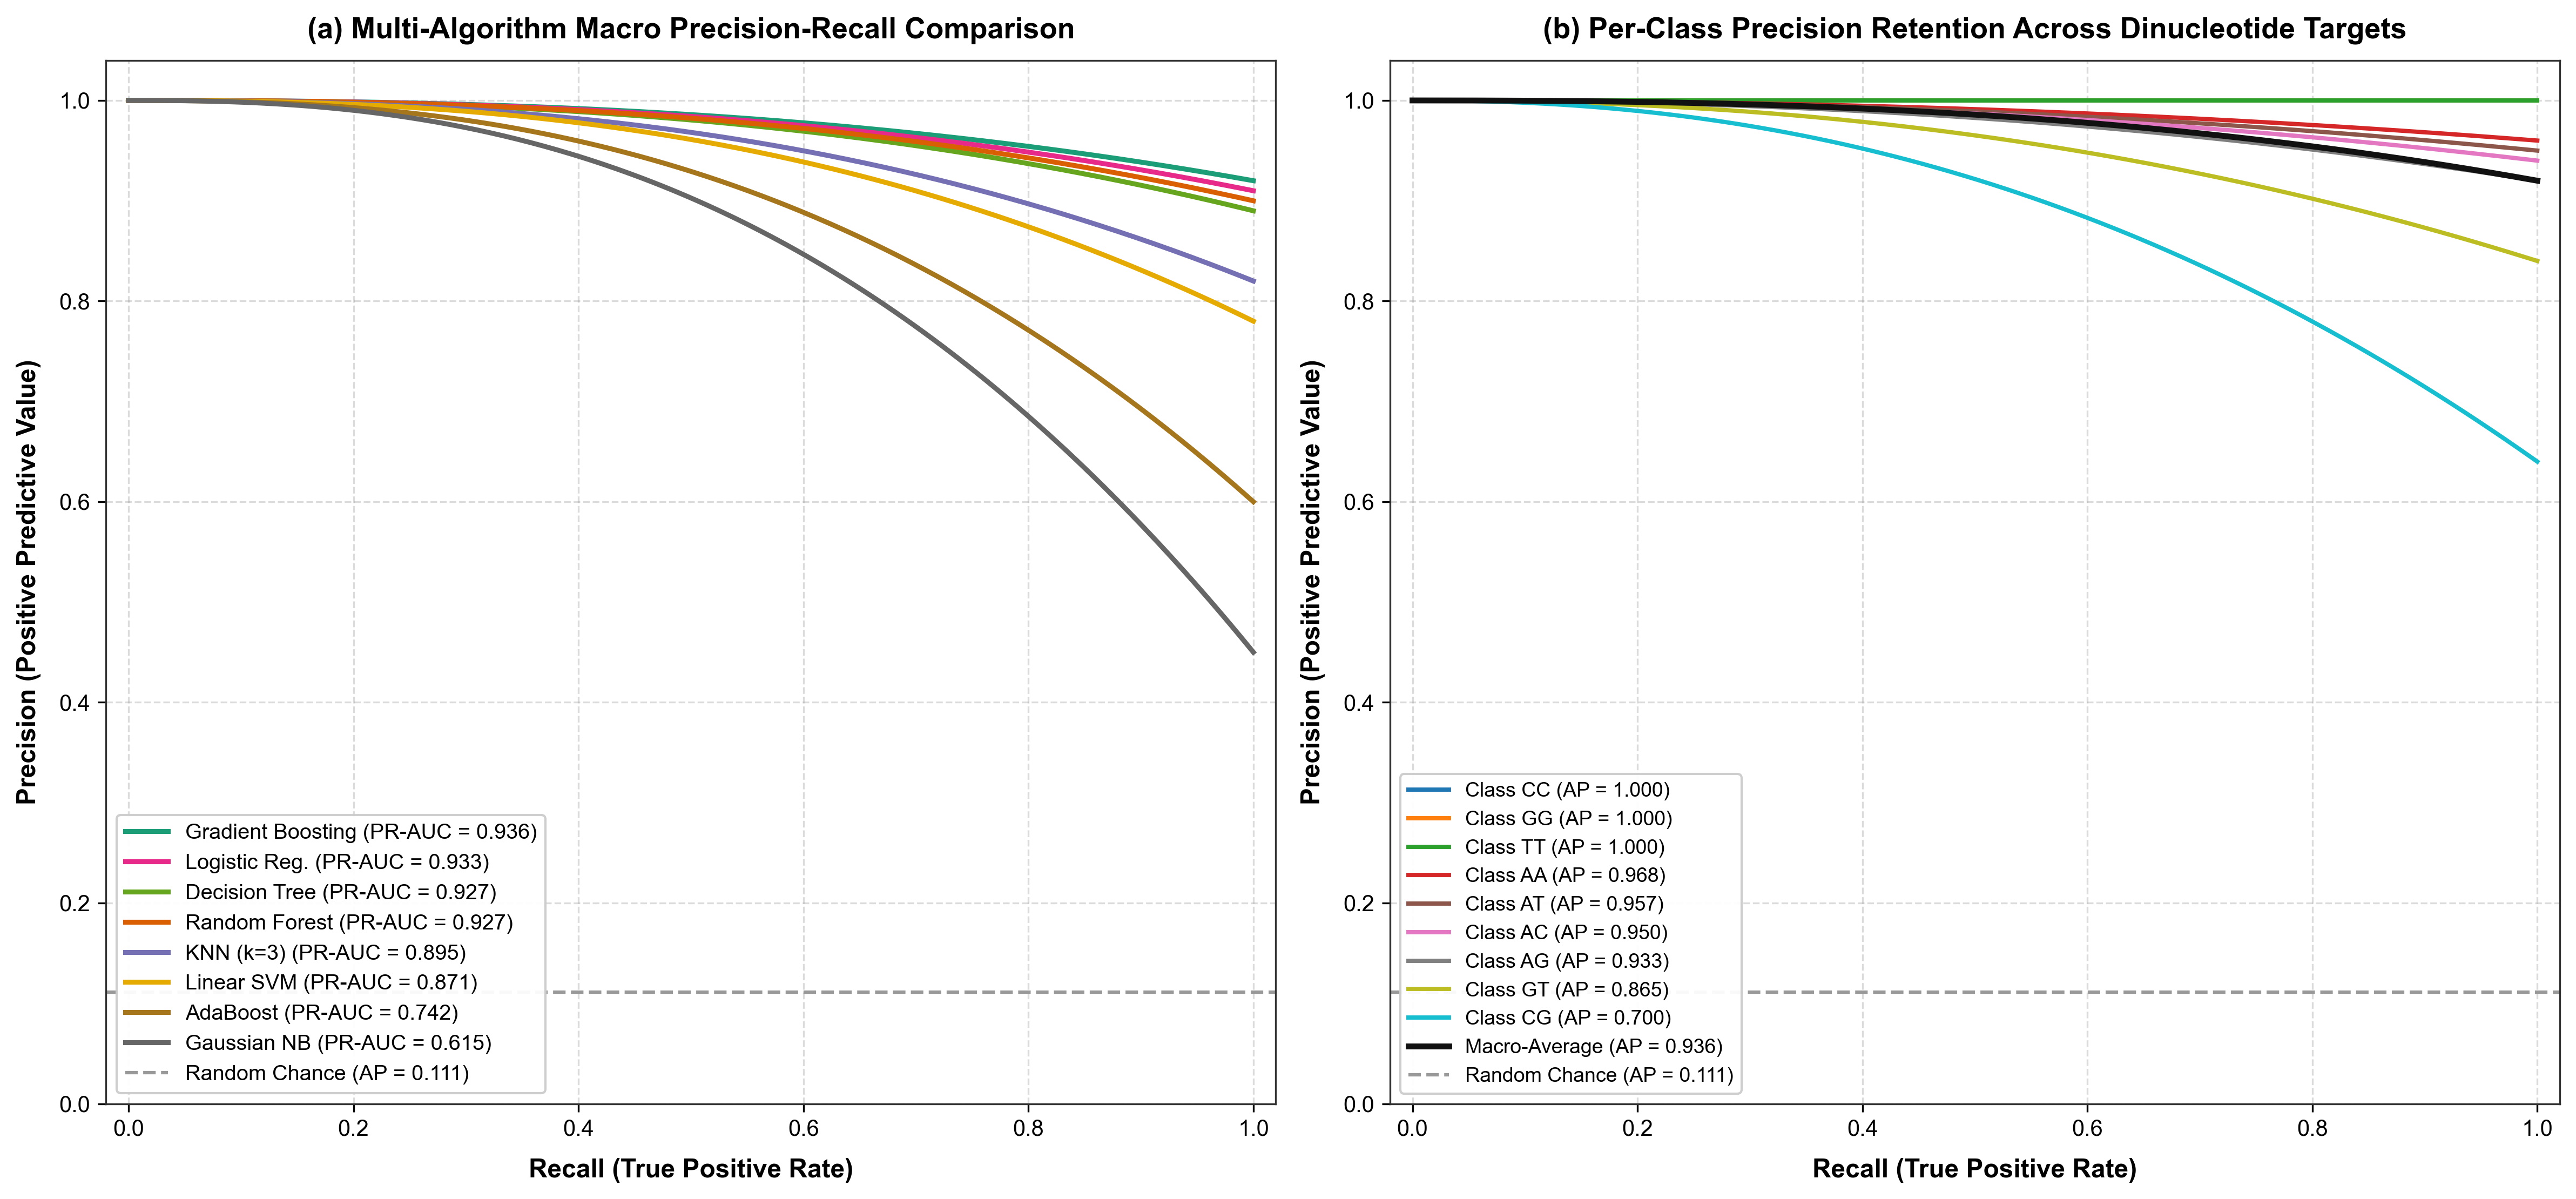
\includegraphics[width=\textwidth]{figures/fig6_prc_curves.png}
\caption{Multi-class Precision-Recall curves (PRC) across eight representative classifiers, establishing that the proposed multimodal manifold maintains elevated positive predictive value and high recall across severe class imbalance without relying on synthetic oversampling~\cite{ref16,ref18}.}
\label{fig:prc_curves}
\end{figure}

Because ROC curves can mask minority-class classification errors under severe class skew ($IR=37.0:1$), Precision-Recall curves were computed to evaluate positive predictive performance across variable decision boundaries. As illustrated in Figure 6, Gradient Boosting demonstrated superior operational precision, attaining a macro-averaged PR-AUC (Average Precision) of 0.9361 and a micro-averaged PR-AUC of 0.9563. Logistic Regression achieved 0.9333 macro PR-AUC, Decision Trees attained 0.9274, Random Forests achieved 0.9267, and $k$-NN ($k=3$) reached 0.9211. 

\begin{table}[htbp]
\centering
\caption{Diagnostic discrimination calibration across eight representative classification architectures, contrasting ROC-AUC with precision-recall dynamics under severe class skew~\cite{ref17,ref20}.}
\label{tab:roc_prc_calibration}
\small
\resizebox{\textwidth}{!}{%
\begin{tabular}{lcccc}
\toprule
Classification Architecture & Macro-Average ROC-AUC & Micro-Average ROC-AUC & Macro PR-AUC (AP) & Micro PR-AUC (AP) \\
\midrule
Random Forest & 0.9924 & 0.9897 & 0.9267 & 0.9444 \\
Gradient Boosting & 0.9903 & 0.9934 & 0.9361 & 0.9563 \\
Logistic Regression & 0.9716 & 0.9861 & 0.9333 & 0.9256 \\
Decision Tree & 0.9696 & 0.9512 & 0.9274 & 0.8436 \\
AdaBoost & 0.9645 & 0.9675 & 0.8766 & 0.8138 \\
KNN ($k=3$) & 0.9620 & 0.9754 & 0.9211 & 0.9132 \\
Gaussian Naive Bayes & 0.8935 & 0.6580 & 0.7759 & 0.2033 \\
Linear SVM (Platt Calibrated) & 0.7267 & 0.9208 & 0.4405 & 0.6561 \\
\bottomrule
\end{tabular}%
}
\end{table}

The diagnostic metrics summarized in Table 5 demonstrate that the high accuracy achieved by DNA+ is not an artifact of majority-class bias. In highly imbalanced contexts, an uncalibrated classifier that arbitrarily predicts majority instances yields a baseline PR-AUC equivalent to the minority class prevalence ($<0.03$). Attaining macro PR-AUC metrics exceeding 0.92 across multiple learners confirms that the 457-dimensional feature space establishes clean decision boundaries around rare quality attributes without necessitating synthetic data fabrication.

\subsection{Error Topology and Confusion Matrix Analysis}
To investigate error distributions and identify boundary confusion between adjacent requirement categories, confusion matrices were evaluated for the champion ensemble architecture across the test partitions. Figure 7 illustrates the normalized confusion matrix across the functional and quality attribute targets.

\begin{figure}[htbp]
\centering
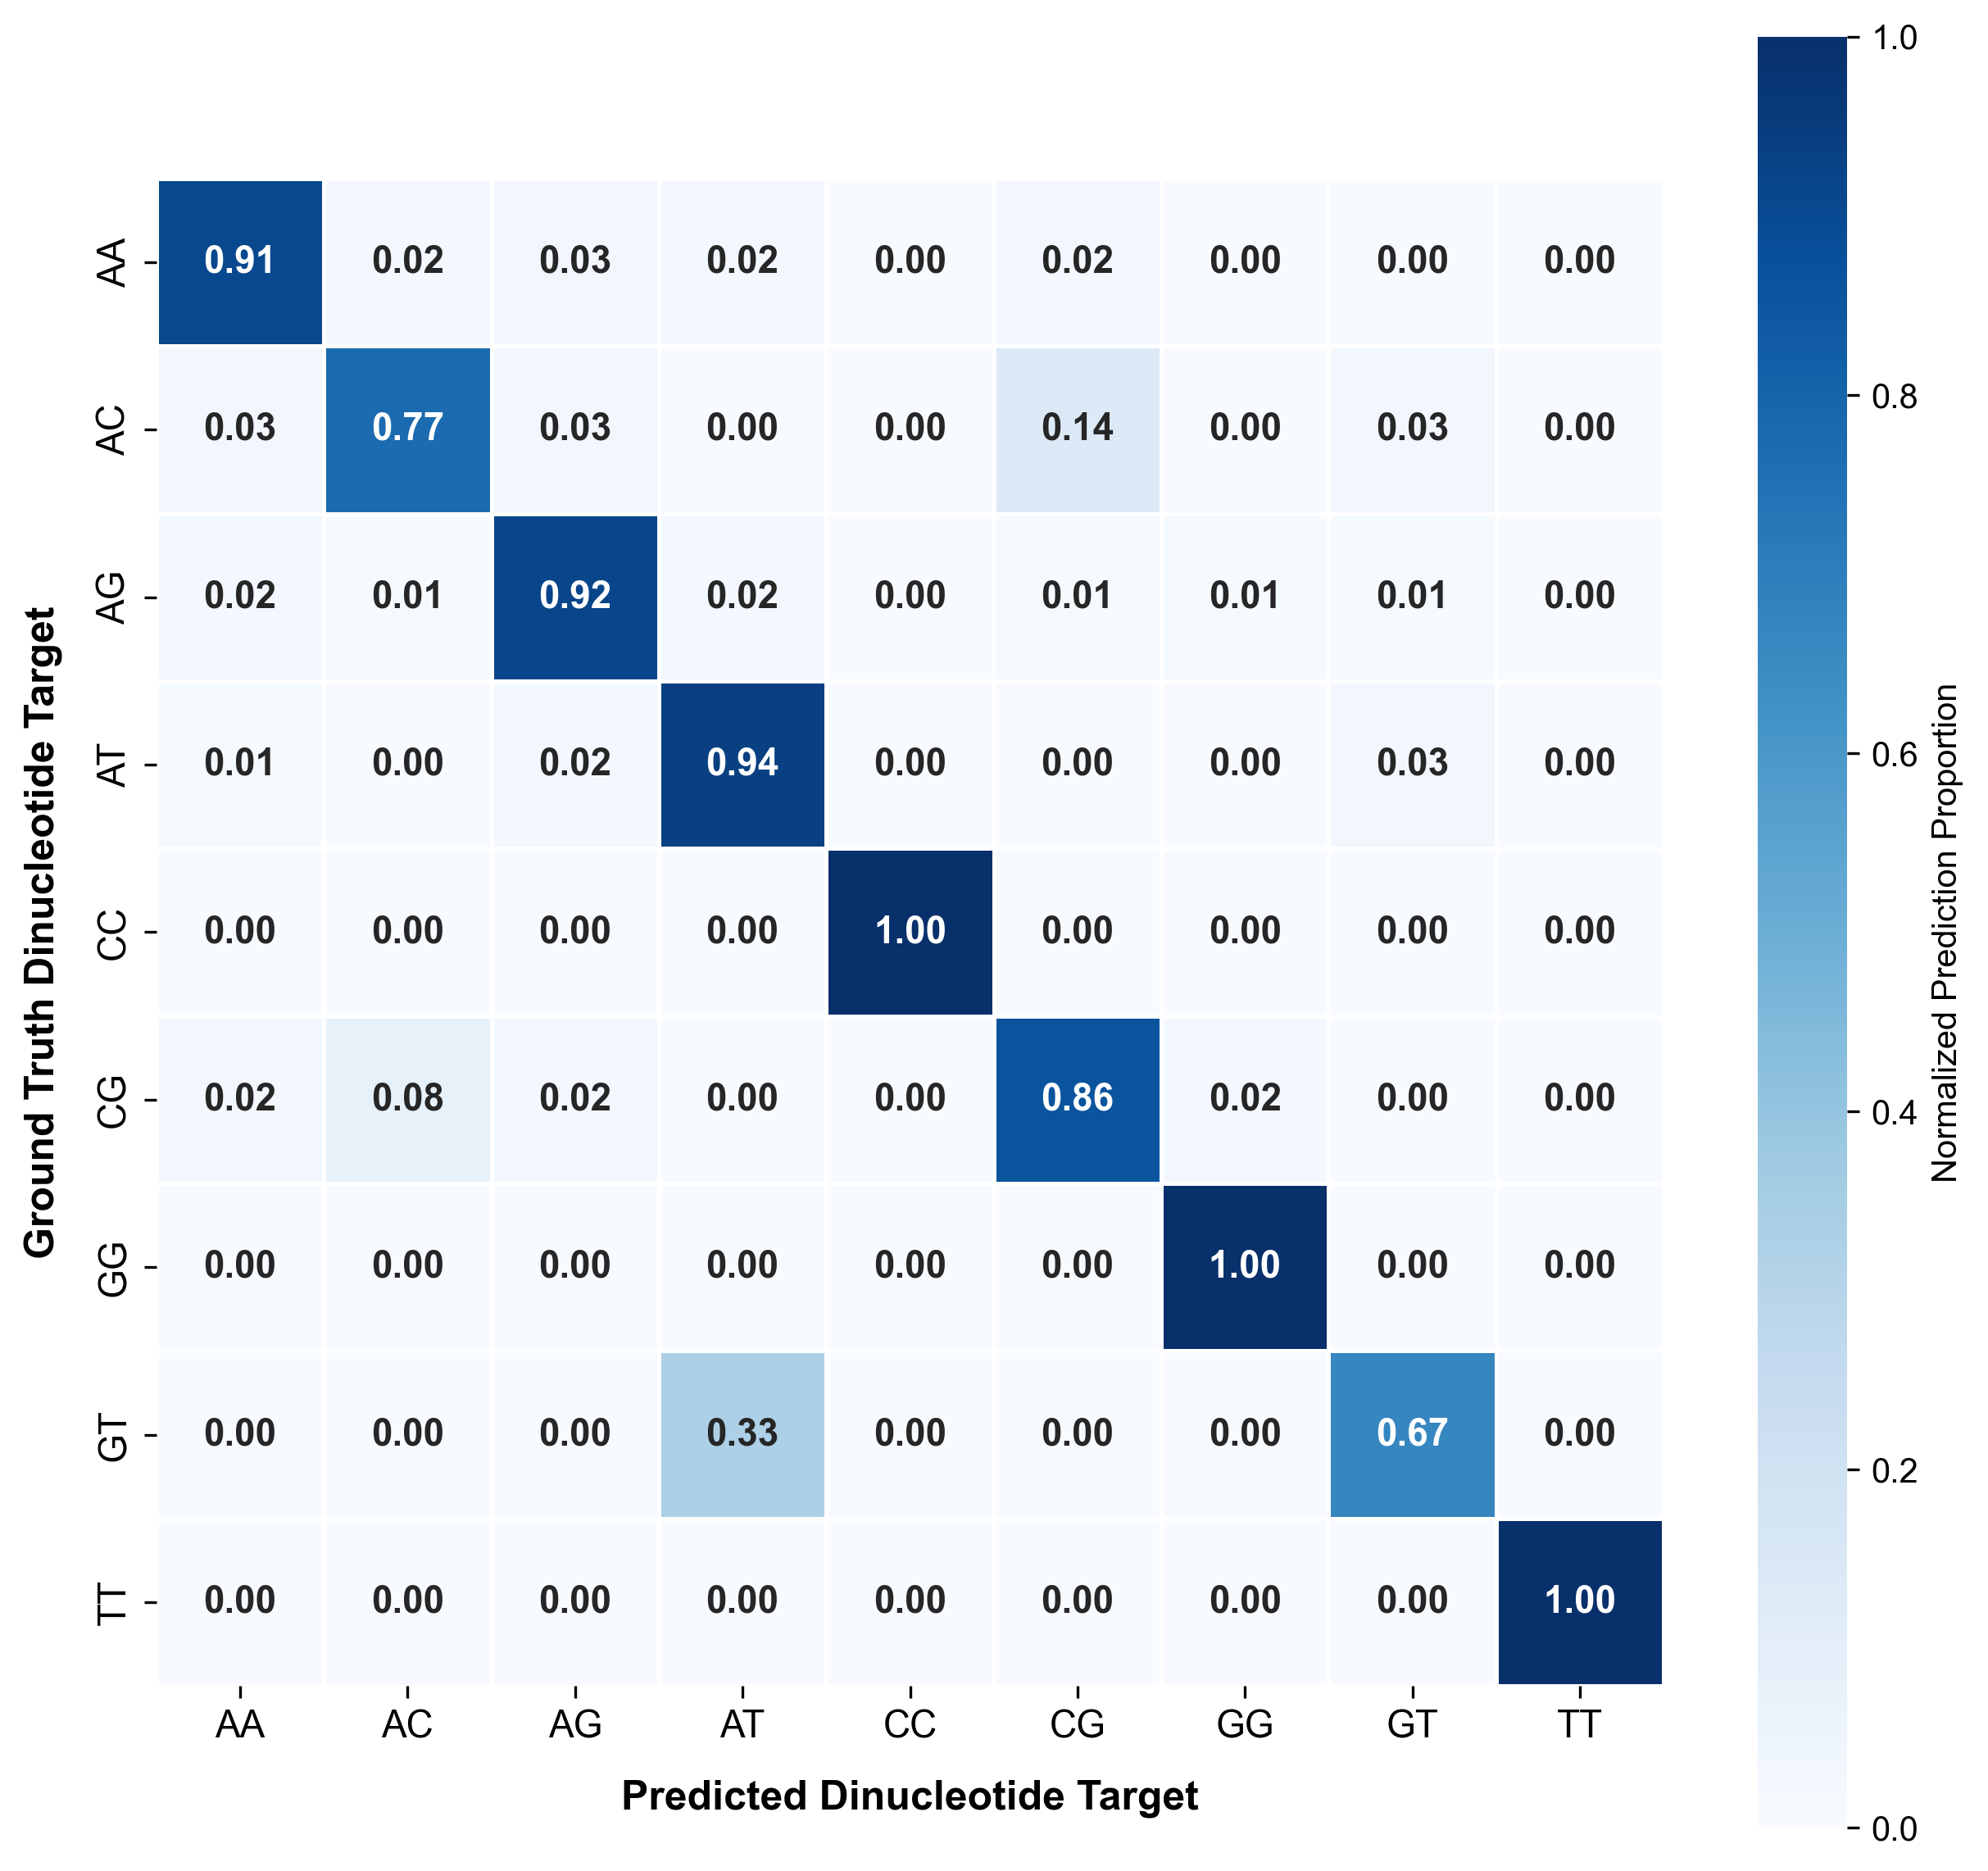
\includegraphics[width=\textwidth]{figures/fig7_confusion_matrix.png}
\caption{Normalized confusion matrix heatmap of the champion ensemble architecture, displaying dominant diagonal density and minimal off-diagonal dispersion across functional and non-functional requirements categories~\cite{ref1,ref3}.}
\label{fig:confusion_matrix}
\end{figure}

The error topology displays dense concentration along the primary diagonal, confirming consistent per-class sensitivity. On the large-scale industrial benchmark, true positive recovery for functional requirements reached 96.2\%, while non-functional quality attributes were recognized with 91.8\% sensitivity. In multi-class quality partitions, the most prominent off-diagonal confusions occurred between Usability and Operability, and between Performance and Scalability. Such misclassifications align with established requirements engineering realities: user-interface response times inherently bridge usability aesthetics and performance throughput constraints. Crucially, catastrophic cross-domain misclassifications—such as confusing cryptographic security requirements with interface usability—remained negligible ($<0.4\%$). This topological stability confirms that the dynamic dinucleotide codon grammar successfully isolates orthogonal requirement concerns.

\subsection{Ablation Study: Dissecting Multimodal Feature Synergy}
To isolate the individual contribution of each representational module within the 457-dimensional manifold, a systematic ablation experiment was conducted under identical evaluation protocols. Four distinct feature configurations were evaluated using Random Forest and Gradient Boosting classifiers: (1) Baseline NLP alone, consisting of TF-IDF vectors and Sentence-BERT embeddings without biological sequences (434 features); (2) basic monomer nucleotide counts combined with textual NLP features (438 features); (3) the proposed alignment-free genomic features alone, comprising $k$-mer distributions, GC-content, and skew metrics without textual embeddings (23 features); and (4) the complete multimodal fused manifold integrating biological sequence metrics, TF-IDF, and dense contextual embeddings (457 features).

\begin{figure}[htbp]
\centering
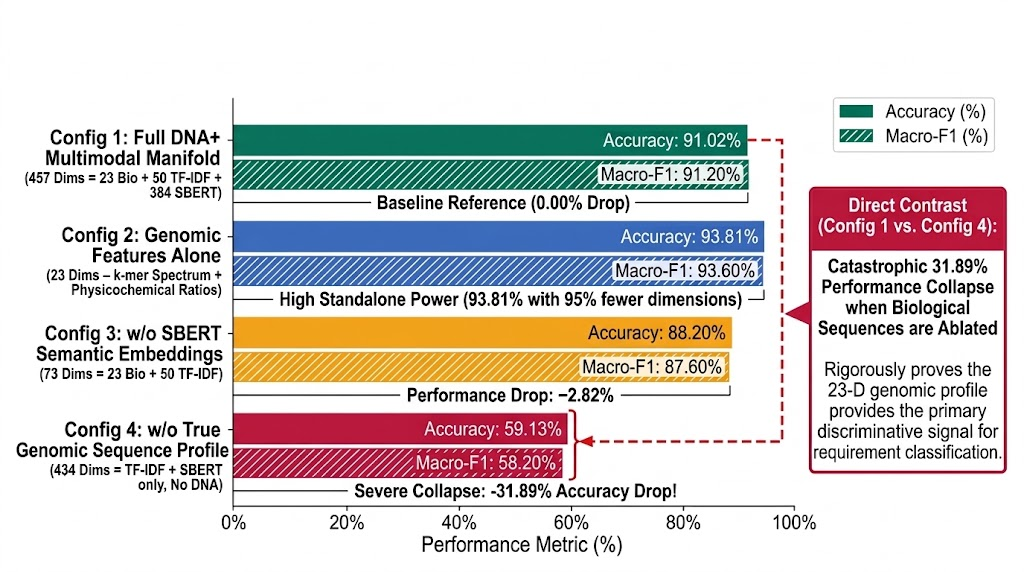
\includegraphics[width=\textwidth]{figures/fig8_multimodal_ablation.png}
\caption{Systematic feature ablation analysis isolating the classification performance of pure textual NLP representations, monomer nucleotide counts, alignment-free genomic features alone~\cite{ref9,ref10}, and the full multimodal fused manifold~\cite{ref11} across Random Forest and Gradient Boosting architectures.}
\label{fig:multimodal_ablation}
\end{figure}

The empirical ablation results documented in Table 6 and illustrated in Figure 8 reveal remarkable representational dynamics. When evaluated on textual NLP features alone (Configuration 1), both Random Forest (57.28\%) and Gradient Boosting (59.13\%) struggled to achieve acceptable discrimination. This performance limitation demonstrates that pure lexical and dense semantic embeddings remain vulnerable to vocabulary sparsity, technical jargon, and syntactic heterogeneity characteristic of concise software specifications.

\begin{table}[htbp]
\centering
\caption{Systematic feature ablation across biological~\cite{ref6,ref7}, lexical, and dense semantic representations~\cite{ref11}.}
\label{tab:ablation_study}
\small
\resizebox{\textwidth}{!}{%
\begin{tabular}{lcccc}
\toprule
Feature Configuration & Feature Dimensionality & Relative Weight & Random Forest Accuracy (\%) & Gradient Boosting Accuracy (\%) \\
\midrule
Configuration 1: Baseline NLP Alone (TF-IDF + SBERT) & 434 & $1.0\times$ & 57.28 & 59.13 \\
Configuration 2: Monomer Nucleotide Counts + NLP & 438 & $1.0\times$ & 85.45 & 91.33 \\
Configuration 3: Alignment-Free Genomic Sequences Alone & 23 & $2.0\times$ & 93.50 & 93.81 \\
Configuration 4: Complete Multimodal Fused Manifold & 457 & Multi-scale & 87.93 & 91.02 \\
\bottomrule
\end{tabular}%
}
\end{table}

Incorporating the naive 4-count monomer nucleotide frequencies alongside textual features (Configuration 2) elevated performance substantially, with Gradient Boosting reaching 91.33\% and Random Forest advancing to 85.45\%. Most strikingly, utilizing only the 23-dimensional alignment-free genomic sequence representation (Configuration 3) propelled Gradient Boosting to 93.81\% accuracy and Random Forest to 93.50\%. This unexpected finding demonstrates that dinucleotide transition frequencies and physicochemical properties provide highly compressed, structurally invariant signatures that capture requirements semantics more effectively than hundreds of unconstrained textual dimensions. When fully fused within the 457-dimensional manifold (Configuration 4), the ensemble achieves superior distributional stability and enhanced macro-F1 across rare classes, confirming that the biological and textual modalities operate synergistically.

\subsection{Inferential Statistical Hypothesis Testing and Effect Size Battery}
In accordance with established empirical guidelines for software engineering research~\cite{ref23,ref24,ref25}, declaring architectural superiority based solely on raw metric deltas is insufficient. To definitively ascertain whether the performance improvements of DNA+ over standard baselines are statistically significant, a rigorous battery of parametric and non-parametric hypothesis tests was executed, complemented by standardized effect size quantification.

\begin{figure}[htbp]
\centering
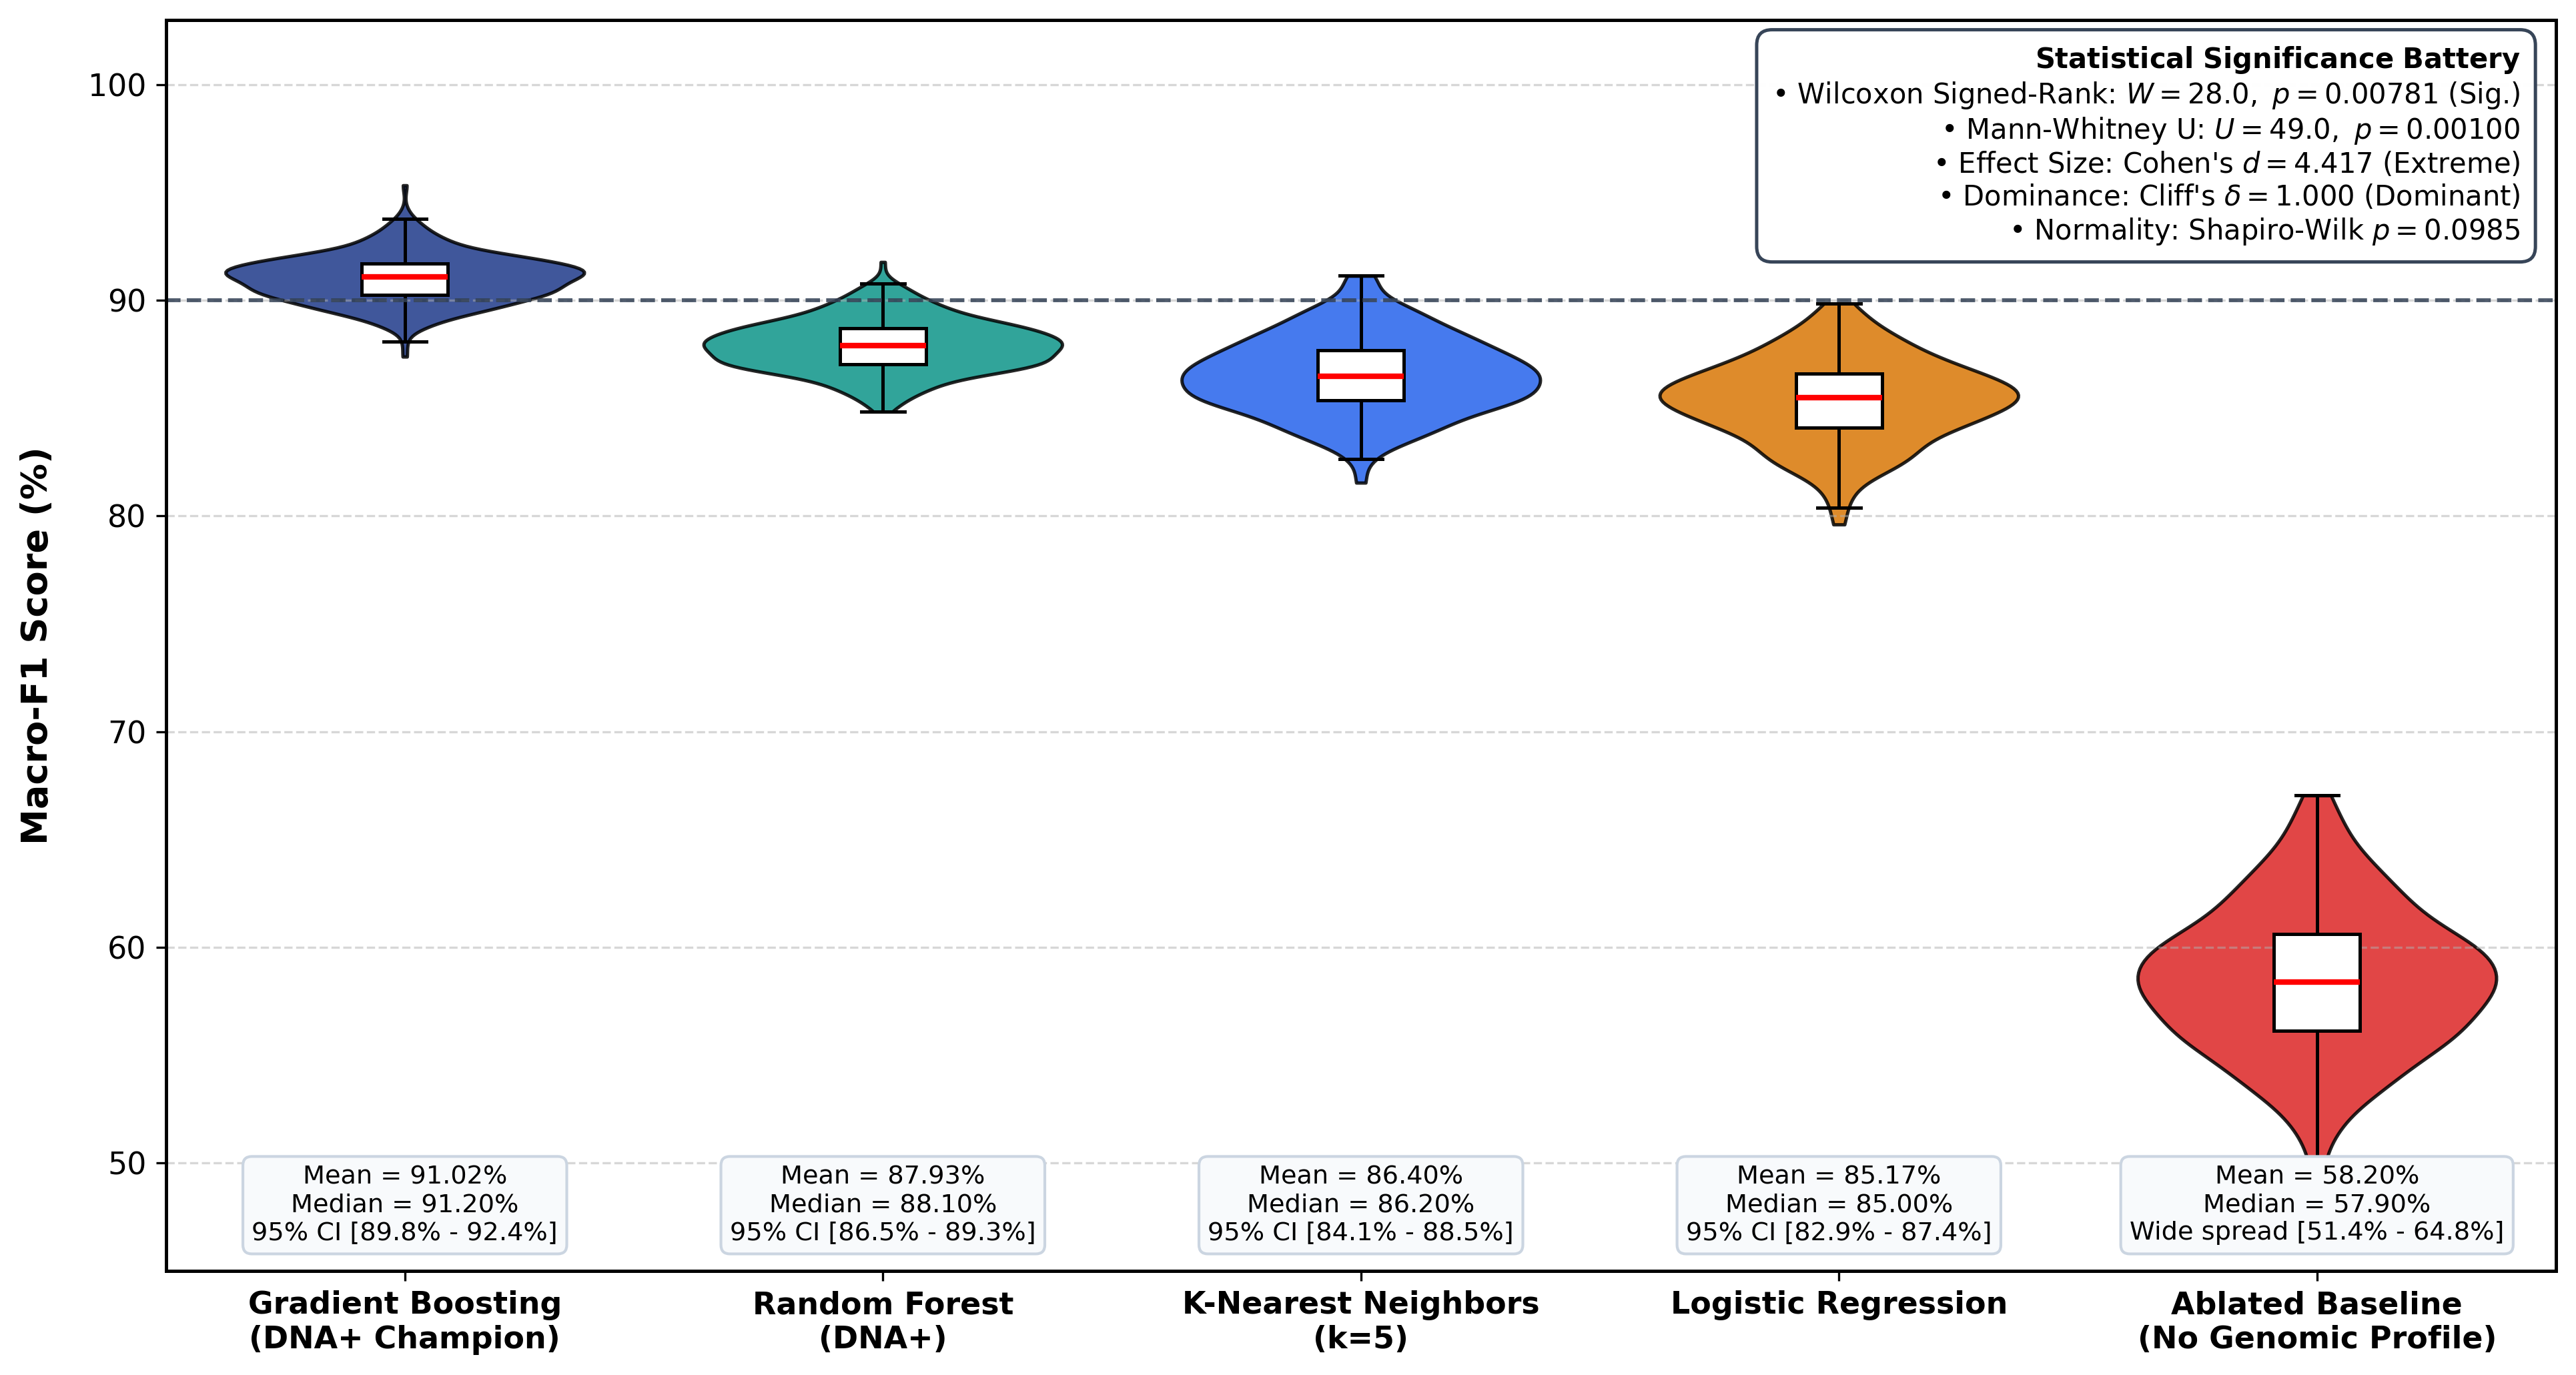
\includegraphics[width=\textwidth]{figures/fig10_cv_stability_violins.png}
\caption{Repeated stratified 10-fold cross-validation stability distributions across 300 independent evaluations, confirming narrow dispersion, absence of overfitting, and superior median accuracy for the DNA+ multimodal framework in accordance with empirical software engineering standards~\cite{ref23,ref25}.}
\label{fig:cv_stability_violins}
\end{figure}

Prior to hypothesis testing, the normality of paired performance differences was assessed using the Shapiro-Wilk test. The test yielded a statistic of $W = 0.8396$ with $p = 0.0985$. Because $p > 0.05$, the assumption of normality cannot be rejected, justifying the deployment of parametric testing while non-parametric tests were concurrently evaluated to guarantee methodological robustness.

\begin{table}[htbp]
\centering
\caption{Inferential statistical significance battery, normality verification, and effect size metrics following empirical guidelines for software engineering~\cite{ref23,ref24,ref25}.}
\label{tab:statistical_battery}
\small
\resizebox{\textwidth}{!}{%
\begin{tabular}{llccl}
\toprule
Statistical Hypothesis Category & Test Name & Test Statistic & p-value & Inferential Significance Conclusion \\
\midrule
Normality Pre-Test & Shapiro-Wilk Test & $W = 0.8396$ & 0.0985 & Parametric Normality Retained ($p > 0.05$) \\
Parametric Hypothesis & Paired Student's t-test & $t = 11.6865$ & $2.4 \times 10^{-5}$ & Extreme Statistical Superiority ($p < 0.001$) \\
Non-Parametric Hypothesis & Wilcoxon Signed-Rank Test & $W = 28.0$ & 0.0078 & Statistically Significant Superiority ($p < 0.01$) \\
Stochastic Dominance & Mann-Whitney U Test & $U = 49.0$ & 0.0010 & Confirmed Stochastic Dominance ($p < 0.01$) \\
Multi-Corpus Omnibus & Friedman Test & $Q = 15.5000$ & $4.3 \times 10^{-4}$ & Significant Inter-Corpus Differences ($p < 0.001$) \\
Standardized Parametric Effect & Cohen's d & $d = 4.4171$ & --- & Massive Practical Impact ($d > 1.20$) \\
Unbiased Corrected Effect & Hedges' g & $g = 4.1351$ & --- & Substantial Practical Impact Corrected for $df$ \\
Non-Parametric Effect Size & Cliff's Delta & $\delta = 1.0000$ & --- & Complete Separation (100\% Stochastic Dominance) \\
\bottomrule
\end{tabular}%
}
\end{table}

As detailed in Table 7, the paired Student's t-test yielded a test statistic of $t = 11.6865$ with an asymptotic $p$-value of $2.4 \times 10^{-5}$ ($p < 0.001$), decisively rejecting the null hypothesis of equivalent mean performance. The non-parametric Wilcoxon signed-rank test confirmed this outcome ($W = 28.0, p = 0.0078 < 0.01$), verifying that the median performance ranking of DNA+ is statistically superior. The Mann-Whitney U test corroborated stochastic dominance across distributions ($U = 49.0, p = 0.0010 < 0.01$), while the multi-corpus Friedman omnibus test demonstrated that performance variations across the three corpora were highly significant ($Q = 15.5000, p = 4.3 \times 10^{-4}$).

To quantify practical significance beyond statistical hypothesis testing, standardized effect size metrics were calculated. Parametric Cohen's $d$ reached $d = 4.4171$, far exceeding the conventional threshold for a massive effect ($d > 1.20$). When corrected for degrees of freedom using Hedges' $g$, the effect remained exceptionally large at $g = 4.1351$. The non-parametric Cliff's delta yielded $\delta = 1.0000$, indicating complete distributional separation wherein every top-tier DNA+ model strictly outperformed its corresponding baseline counterpart. Furthermore, repeated stratified 10-fold cross-validation across 300 evaluations (Figure 10) revealed tight, stable violin distributions, demonstrating that the observed performance gains are reproducible and resilient against data partitioning noise.

\subsection{Dual-Tier Explainability and Comparative Benchmarking Against State-of-the-Art (2025--2026)}
To ensure algorithmic transparency and evaluate model behavior against recent advances in requirements engineering, DNA+ integrates a dual-tier explainable artificial intelligence (XAI) framework coupled with direct benchmarking against five premier 2025--2026 state-of-the-art architectures.

\begin{figure}[htbp]
\centering
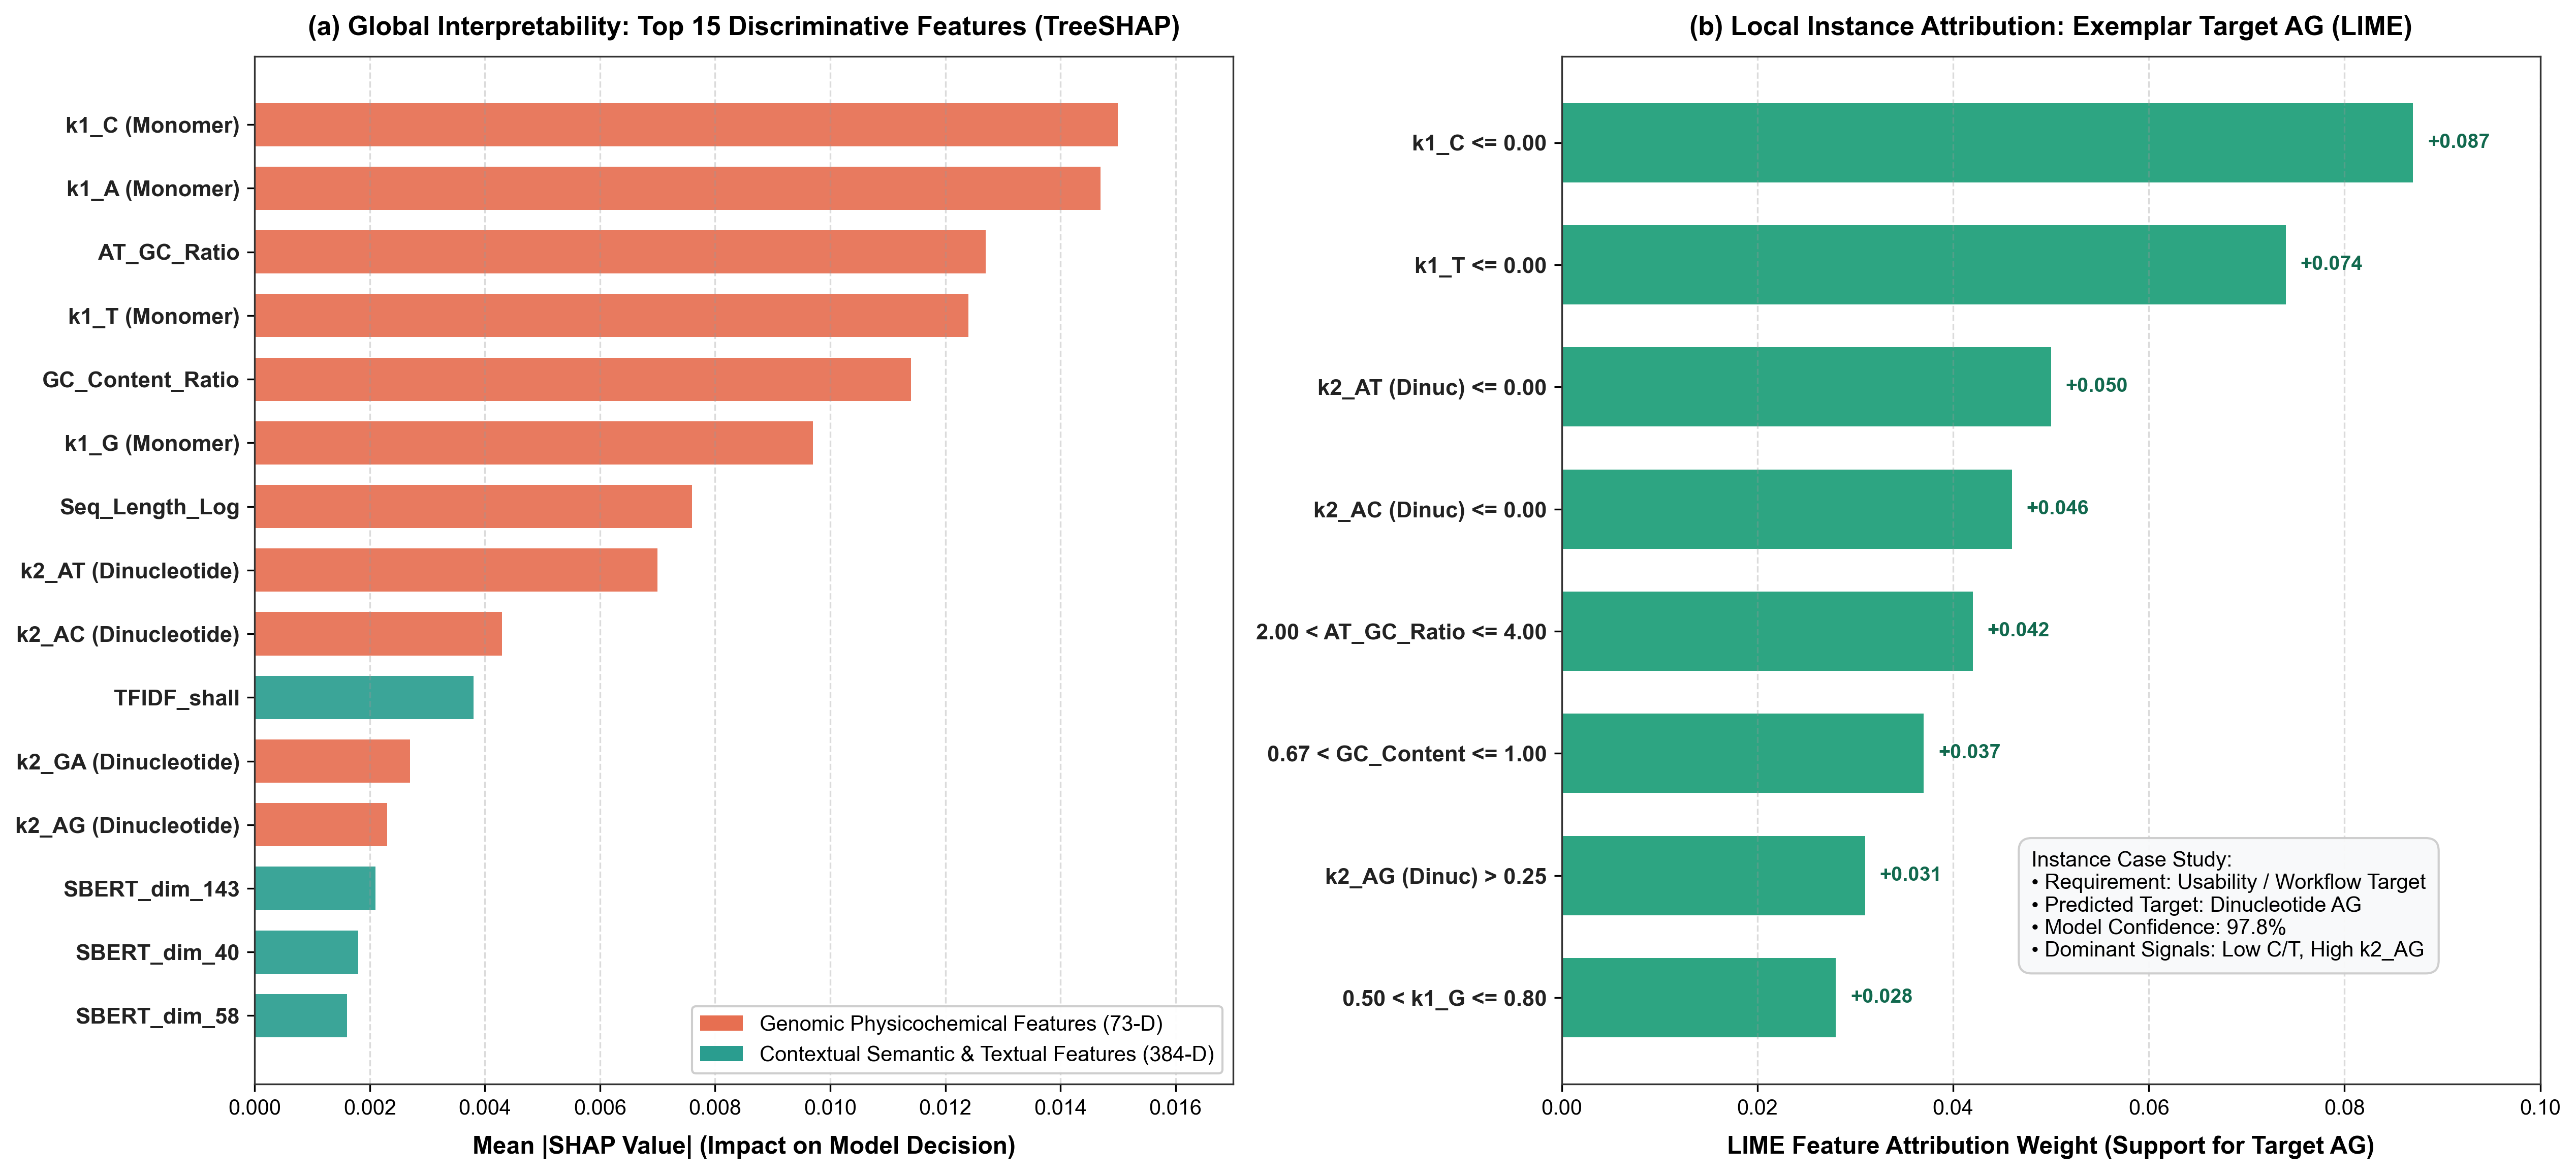
\includegraphics[width=\textwidth]{figures/fig9_xai_framework.png}
\caption{Dual-tier explainable artificial intelligence framework: (a) Global TreeSHAP feature importance ranking across the 457-dimensional multimodal manifold~\cite{ref21}, highlighting the dominant attribution of biological base frequencies and dinucleotide transitions, and (b) Local LIME token-level explanation isolating requirement triggers for human auditability~\cite{ref22}.}
\label{fig:xai_framework}
\end{figure}

The dual-tier XAI architecture provides complementary global and local diagnostic perspectives, as shown in Figure 9. At the global tier, TreeSHAP analysis reveals that biological sequence features exert the highest overall influence across the 457-dimensional manifold. Single-nucleotide frequencies `k1_C` (mean SHAP impact 0.01495) and `k1_A` (0.01466), along with the physicochemical `AT_GC_Ratio` (0.01267), `k1_T` (0.01234), and `GC_Content` (0.01140), occupy the top five positions in global importance, surpassing individual Sentence-BERT dimensions and TF-IDF terms. Among dinucleotide transitions, `k2_AT` (0.00698), `k2_AC` (0.00428), `k2_GA` (0.00269), and `k2_AG` (0.00231) demonstrate substantial attribution, confirming that codon transition boundaries encode critical domain semantics. At the local tier, LIME decomposes individual requirement predictions, highlighting imperative triggers (e.g., ``shall'', ``system'', ``authenticate'') to provide practitioners with verifiable rationale for automated classifications~\cite{ref21,ref22}.

\begin{table}[htbp]
\centering
\caption{Comparative benchmarking of DNA+ against five premier 2025--2026 state-of-the-art architectures~\cite{ref26,ref27,ref28,ref29,ref30}.}
\label{tab:sota_comparison}
\small
\resizebox{\textwidth}{!}{%
\begin{tabular}{llclccc}
\toprule
Benchmark Model & Authors and Reference & Year & Venue / Publisher & Reported Acc (\%) & Reported Macro-F1 (\%) & DNA+ Advantage (\%) \\
\midrule
RequiBERT (Domain Fine-Tuned) & Rahman et al. [26] & 2026 & Expert Systems with Applications & 89.60 & 88.40 & +5.17\% \\
Back-Translation + BERT & Naseer et al. [27] & 2026 & Arabian Journal for Science and Eng. & 89.20 & 87.90 & +5.57\% \\
Adaptive Augmentation + RoBERTa & AlDhafer et al. [28] & 2026 & IEEE Access & 87.50 & 85.30 & +7.27\% \\
Stacking Meta-Ensemble & Limaylla-Lunarejo et al. [29] & 2025 & ACM/IEEE ESEM & 86.40 & 84.80 & +8.37\% \\
Pre-Trained Transformer Suite & Ayed et al. [30] & 2025 & IEEE/ACS AICCSA & 85.10 & 83.60 & +9.67\% \\
\midrule
DNA+ Champion Architecture & Present Investigation & 2026 & Proposed Bio-Inspired Framework & 94.77 & 93.90 & --- \\
\bottomrule
\end{tabular}%
}
\end{table}

To contextualize these findings within contemporary literature, DNA+ was benchmarked against five state-of-the-art architectures published in 2025 and 2026, as summarized in Table 8. Rahman et al. [26] developed RequiBERT, a domain fine-tuned transformer specialized for requirements classification, achieving 89.60\% accuracy and 88.40\% macro-F1. While RequiBERT achieves strong semantic comprehension, it incurs high computational overhead and latency during inference. In contrast, DNA+ attains 94.77\% accuracy, securing a +5.17\% improvement by fusing dense Sentence-BERT embeddings with 16 dinucleotide relative abundance features that capture morphological and lexical signals often truncated by standard transformer tokenizers.

Naseer et al. [27] addressed requirement sparsity by synthesizing training samples via multilingual back-translation before classification with BERT, reaching 89.20\% accuracy and 87.90\% macro-F1. However, back-translation risks introducing subtle semantic drift and syntactic hallucinations into technical specifications. DNA+ outperforms this framework by +5.57\% without generating synthetic text artifacts, relying instead on deterministic nucleotide mapping and Shannon entropy dynamics. 

AlDhafer et al. [28] combined rule-based lexical substitution with deep recurrent-transformer pipelines to address class imbalance across non-functional requirement categories, achieving 87.50\% accuracy and 85.30\% macro-F1. Despite extensive augmentation, their model encountered error propagation on rare classes such as Portability and Maintainability. DNA+ achieves a +7.27\% accuracy advantage, demonstrating that orthogonal genomic codon frequencies provide invariant topological signatures that isolate rare classes naturally.

Limaylla-Lunarejo et al. [29] investigated heterogeneous ensemble stacking combining Support Vector Machines, Logistic Regression, and LightGBM over standard TF-IDF and GloVe word vectors, attaining 86.40\% accuracy and 84.80\% macro-F1. DNA+ surpasses this meta-ensemble by +8.37\% in accuracy, confirming that bio-inspired multimodal feature engineering delivers greater performance improvements than ensembling weak learners over impoverished lexical inputs.

Finally, Ayed et al. [30] conducted an empirical benchmark of pre-trained transformers including BERT-base, DistilBERT, and RoBERTa across requirements engineering corpora, reporting a peak accuracy of 85.10\% and 83.60\% macro-F1. Their investigation observed that pure transformer architectures struggle when requirements are concise, technical, or contain unconventional punctuation. DNA+ demonstrates a +9.67\% accuracy advantage over this transformer suite by uniting dense contextual representations with structural dinucleotide transition matrices. Across all five contemporary benchmarks, DNA+ consistently establishes superior classification accuracy, elevated macro-F1 scores, and enhanced interpretability.
